\documentclass{article}

\usepackage[utf8]{inputenc}

\usepackage{nicefrac}
\usepackage{amssymb, amsmath, amsfonts}
\usepackage{amsthm}
\usepackage{tikz}
\usetikzlibrary{matrix,shapes,arrows}
\usepackage{pgfplots}
\usepgfplotslibrary{groupplots}
\usepackage[a4paper, margin=1in]{geometry}

\newtheorem{proposition}{Proposition}
\newtheorem{theorem}{Theorem}
\newtheorem{definition}{Definition}
\newtheorem{lemma}{Lemma}
\newtheorem{conjecture}{Conjecture}
\newtheorem{corollary}{Corollary}
\newtheorem{remark}{Remark}
\newtheorem{assumption}{Assumption}

\newlength\figureheight
\newlength\figurewidth
\setlength\figureheight{5cm}
\setlength\figurewidth{14cm}

\newcommand{\tikzdir}[1]{tikz/#1.tikz}
\newcommand{\inputtikz}[1]{\input{\tikzdir{#1}}}

\DeclareMathOperator*{\argmin}{arg\; min}     % argmin
\DeclareMathOperator*{\argmax}{arg\; max}     % argmax
\DeclareMathOperator*{\tr}{tr}     % trace
\DeclareMathOperator{\Cov}{Cov}
\DeclareMathOperator{\logdet}{log\;det}

\title{EE3011 Modeling and Control\\Tutorial 12: Controller Design}
\date{}
\begin{document} \maketitle
\begin{enumerate}
\item A feedback control system is as shown in Figure~\ref{fig:1}. 
  \begin{figure}[h]
    \centering
    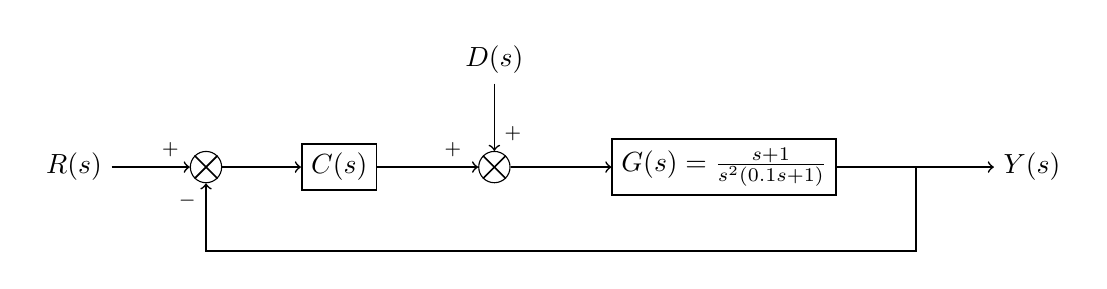
\begin{tikzpicture}
      \tikzstyle{point} = [coordinate]
      \tikzstyle{box} = [rectangle, draw, semithick]
      \matrix[row sep = 7mm, column sep = 10mm]{
        &
        &
        &
        \node (d) {$D(s)$};&
        &
        &
        \\
        % first row
        \node (p1) [] {$R(s)$};&
        \node (p2) [circle,draw,inner sep=4pt] {};&
        \node (outer) [box] {$C(s)$};&
        \node (p3) [circle,draw,inner sep=4pt] {};&
        \node (inner) [box] {$G(s)=\frac{s+1}{s^2(0.1s+1)}$};&
        \node (p5) [point] {};&
        \node (p6) [] {$Y(s)$};\\
        % third row
        &
        \node (p9) [point] {};&
        &
        &
        &
        \node (p10) [point] {};&
        \\
      };
      \draw [semithick,->] (p1)--node[near end, above]{\scriptsize{$+$}} (p2);
      \draw [semithick,->] (p2)--(outer);
      \draw [semithick,->] (outer)--node[near end,above]{\scriptsize{$+$}} (p3);
      \draw [semithick,->] (p3)--(inner);
      \draw [semithick,->] (d)--node[near end,right]{\scriptsize{$+$}} (p3);
      \draw [semithick,->] (inner)--(p5)--(p6);
      \draw [semithick,->] (p5)--(p10)--(p9)--node[near end, left]{\scriptsize{$-$}} (p2);
      \draw [semithick] (p2.north east)--(p2.south west);
      \draw [semithick] (p2.south east)--(p2.north west);
      \draw [semithick] (p3.north east)--(p3.south west);
      \draw [semithick] (p3.south east)--(p3.north west);
    \end{tikzpicture}
    \caption{Block Diagram\label{fig:1}}
  \end{figure}
  \begin{enumerate}
  \item Given the Bode plots of $G(s)$ in Fig~\ref{fig:bode1}, determine a proportional controller, i.e., $C(s) = K$, such that the gain crossover frequency of the system is $10$ rad/s. Is the system closed-loop stable?
\begin{figure}[ht]
  \centering
  \inputtikz{Tut121}
  \caption{\label{fig:bode1}}
\end{figure}
  \item Let the compensator $C(s) = K \frac{Ts+1}{\gamma Ts+1}$. With the value of $K$ obtained in (a), find the suitable parameter $T$ and $\gamma$, such that the gain crossover frequency of the system is at least $10$ rad/s and the phase margin of the system is at least $60^\circ$.
  \item To meet the disturbance rejection requirement, a student proposes to use a PI controller. Can this strategy achieve the specifications given in (b)? Explain.
  \end{enumerate}

\item Consider the control system as shown in Figure~\ref{fig:2}. 
  \begin{figure}[h]
    \centering
    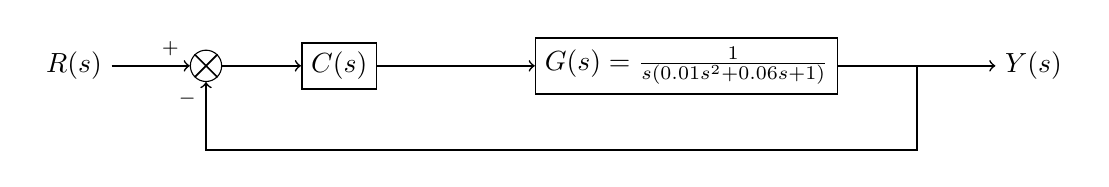
\begin{tikzpicture}
      \tikzstyle{point} = [coordinate]
      \tikzstyle{box} = [rectangle, draw, semithick]
      \matrix[row sep = 7mm, column sep = 10mm]{
        % first row
        \node (p1) [] {$R(s)$};&
        \node (p2) [circle,draw,inner sep=4pt] {};&
        \node (outer) [box] {$C(s)$};&
        \node (p3) [point] {};&
        \node (inner) [box] {$G(s) = \frac{1}{s(0.01s^2+0.06s+1)}$};&
        \node (p5) [point] {};&
        \node (p6) [] {$Y(s)$};\\
        % third row
        &
        \node (p9) [point] {};&
        &
        &
        &
        \node (p10) [point] {};&
        \\
      };
      \draw [semithick,->] (p1)--node[near end, above]{\scriptsize{$+$}} (p2);
      \draw [semithick,->] (p2)--(outer);
      \draw [semithick,->] (outer)--(p3)--(inner);
      \draw [semithick,->] (inner)--(p5)--(p6);
      \draw [semithick,->] (p5)--(p10)--(p9)--node[near end, left]{\scriptsize{$-$}} (p2);
      \draw [semithick] (p2.north east)--(p2.south west);
      \draw [semithick] (p2.south east)--(p2.north west);
    \end{tikzpicture}
    \caption{Block Diagram\label{fig:2}}
  \end{figure}

  Given the Bode plots of $G(s)$ in Figure~\ref{fig:bode2}, design a suitable compensator $G(s)$ to meet the following specifications:
\begin{figure}[ht]
  \centering
  \inputtikz{Tut122}
  \caption{\label{fig:bode2}}
\end{figure}
  \begin{enumerate}
  \item The steady-state error due to a unit-ramp input is less than or equals to $0.1$
  \item The gain crossover frequency is less than or equal to $6$ rad/s
  \item The phase margin of the system is at least $50^\circ$
  \end{enumerate}
  If there exists a delay of $0.2$ sec in $G(s)$, can the compensator designed maintain the stability of the system?
\item An engineer conducts a step response test for a furnace temperature system. The steady-state input is $100$. At time $0$, the input is changed to $110$ and stay constant for the rest of the experiment. The corresponding process reaction curve is shown in Figure~\ref{fig:step}. The red dashed line corresponds to the maximum slope tangent line. Process the data and produces the tuning parameters for a PI controller.
  \begin{figure}[ht]
    \centering
    \inputtikz{Tut123}
    \caption{\label{fig:step}}
  \end{figure}
  \newpage
\item Consider the control system as shown in Figure~\ref{fig:4}. Using the Ziegler-Nichols tuning rule, determine the values of $K_p$, $T_i$ and $T_d$.
  \begin{figure}[h]
    \centering
    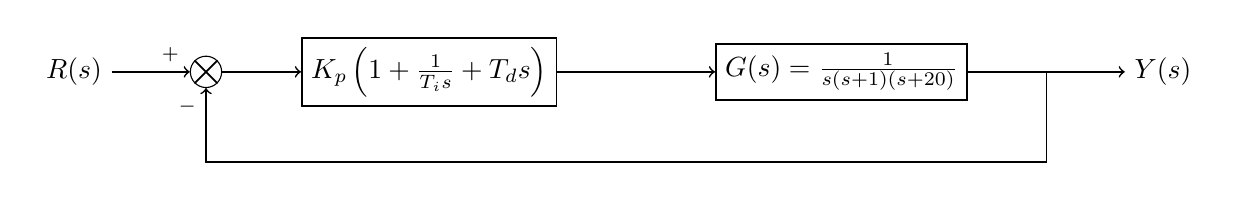
\begin{tikzpicture}
      \tikzstyle{point} = [coordinate]
      \tikzstyle{box} = [rectangle, draw, semithick]
      \matrix[row sep = 7mm, column sep = 10mm]{
        % first row
        \node (p1) [] {$R(s)$};&
        \node (p2) [circle,draw,inner sep=4pt] {};&
        \node (outer) [box] {$K_p\left(1+\frac{1}{T_is}+T_ds\right)$};&
        \node (p3) [point] {};&
        \node (inner) [box] {$G(s) = \frac{1}{s(s+1)(s+20)}$};&
        \node (p5) [point] {};&
        \node (p6) [] {$Y(s)$};\\
        % third row
        &
        \node (p9) [point] {};&
        &
        &
        &
        \node (p10) [point] {};&
        \\
      };
      \draw [semithick,->] (p1)--node[near end, above]{\scriptsize{$+$}} (p2);
      \draw [semithick,->] (p2)--(outer);
      \draw [semithick,->] (outer)--(p3)--(inner);
      \draw [semithick,->] (inner)--(p5)--(p6);
      \draw [semithick,->] (p5)--(p10)--(p9)--node[near end, left]{\scriptsize{$-$}} (p2);
      \draw [semithick] (p2.north east)--(p2.south west);
      \draw [semithick] (p2.south east)--(p2.north west);
    \end{tikzpicture}
    \caption{Block Diagram\label{fig:4}}
  \end{figure}
\end{enumerate}


\end{document}
%%% Local Variables:
%%% TeX-command-default: "Latexmk"
%%% End:
